\documentclass[review]{elsarticle}

\usepackage[colorlinks]{hyperref}
\usepackage[colorinlistoftodos]{todonotes}
\usepackage{verbatim}
\usepackage[utf8]{inputenc}
\usepackage[T1]{fontenc}
\usepackage{adjustbox}
\usepackage{multirow}
\usepackage{longtable}
\usepackage{booktabs}
\usepackage{lineno,hyperref}
\modulolinenumbers[5]

\journal{CRHR Research Reports}

%%%%%%%%%%%%%%%%%%%%%%%
%% Elsevier bibliography styles
%%%%%%%%%%%%%%%%%%%%%%%
%% To change the style, put a % in front of the second line of the current style and
%% remove the % from the second line of the style you would like to use.
%%%%%%%%%%%%%%%%%%%%%%%

%% Numbered
%\bibliographystyle{model1-num-names}

%% Numbered without titles
%\bibliographystyle{model1a-num-names}

%% Harvard 
%\bibliographystyle{model2-names.bst}\biboptions{authoryear}

%% Vancouver numbered
%\usepackage{numcompress}\bibliographystyle{model3-num-names}

%% Vancouver name/year
%\usepackage{numcompress}\bibliographystyle{model4-names}\biboptions{authoryear}

%% APA style
\bibliographystyle{model5-names}\biboptions{authoryear}

%% AMA style
%\usepackage{numcompress}\bibliographystyle{model6-num-names}

%% `Elsevier LaTeX' style
%\bibliographystyle{elsarticle-num}
%%%%%%%%%%%%%%%%%%%%%%%

\begin{document}

\begin{frontmatter}

\title{Morphological Variation in Three-Dimensional Printed Replicas}

%% Group authors per affiliation:
\author{Robert Z. Selden, Jr.\textsuperscript{a,b}*, Bernard K. Means\textsuperscript{a,c}, Kreg Mosier\textsuperscript{d}, and Edward G. Iglesias\textsuperscript{d}}
\address[1]{Heritage Research Center, Stephen F. Austin State University, US}
\address[2]{Cultural Heritage Department, Jean Monnet University, FR}
\address[3]{Virtual Curation Laboratory, Virginia Commonwealth University, US}
\address[4]{Ralph W. Steen Library, Stephen F. Austin State University, US}
\cortext[cor1]{Corresponding author, Robert Z. Selden, Jr. (zselden@sfasu.edu)}

\begin{abstract}
Employed primarily for outreach and education, the three-dimensional (3D) printer used in this analysis provides a means of producing tangible models of fragile and restricted-use specimens for students from a wide variety of disciplines, and is used here to produce prints associated with historic and prehistoric cultural objects. Recognizing that inconsistencies occur in 3D prints due to environmental variables, this exploratory effort was aimed at identifying the geometry that deviates most from the original scan data. A total of five replicas were printed then compared by calculating the gap distance between the nominal (original scan data) and measured data (scan of 3D printed replica) in Geomagic Control X. Results indicate that computer-aided inspection may prove useful in the refinement of 3D printing work flows, finishing, and the iterative refinement of 3D printer settings for specific real-world education- and outreach-based endeavors.
\end{abstract}

\begin{keyword}
3D \sep scanning \sep printing \sep computer aided inspection \sep museum studies
\end{keyword}

\end{frontmatter}

\section{Introduction}

Three-dimensional (3D) prints of archaeological specimens have been used for research \citep{RN11511,RN5942,RN5941,RN5943}, as well as outreach and education purposes \citep{RN11509,RN5944,RN5945,RN11508,RN11505}. The addition of open access 3D meshes to digital repositories and archives \citep{RN5932,RN11507,RN5922} provides access to artifacts from across the world; many of which are available for download as 3D print-ready files. Those investigators adding to the growing corpus of accessible meshes are to be applauded, as their efforts continue to increase global exposure to the history and prehistory of different regions and cultures, adding digital and---when printed or manufactured---physical access to important collections of artifacts to a wide range of students and the general public.

In some ways, the full potential of many 3D digitally documented archaeological remains, ironically, may not be realized until they are replicated through 3D printing. Accurate identification of some artifacts and ecofacts, bone in particular, is most readily achieved through examination of physical objects, either real or replica. The use of 3D printed artifact and ecofact replicas aids archaeologists in meeting their ethical obligations to present their findings and interpretations to the general public, who directly or indirectly support their research, while simultaneously meeting ethical obligations to ensure that those collections are preserved for future generations \citep{RN725}.

There are hundreds of 3D printers available to consumers, which vary from kits requiring considerable assembly to plug-and-play options. Prices also vary considerably, ranging from under one hundred dollars to those costing in the thousands. 3D Hubs, a network of 3D printer owners, evaluated over 400 different 3D printers for 2016 \citep{RN11513} and the number of new 3D printers coming to the market changes on an almost weekly basis. Fused deposition modeling (FDM) printers are the most common because they are simple to operate and are less costly than other 3D printers. FDM printers basically work in the same fashion. Plastic filament is fed from a spool through a super-heated head, which melts the filament into a thin strand. The head moves in patterns dictated by the 3D file, laying down layer upon layer to create the object. For irregular objects, additional plastic supports are generated to ensure that objects do not fall or incur other printing failures \citep{RN5946,RN5947}. The two primary types of filament used in FDM printers are Acrylonitrile Butadiene Styrene (ABS) and Polylactic Acid (PLA) \citep{RN11516,RN11515,RN11514}. The latter exhibits little shrinking relative to the former. An additional major printer technology involves the use of optical power to cure liquid resin into a solid object. Resin-based printers tend to be more expensive, and can be more difficult to operate, but the prints are of high quality and more precise than FDM printers \citep{RN11513}. 

While accuracy is less of a concern for outreach, the utility of prints remains high \citep{RN5938,RN5939}. Replicas can be scaled up or down, allowing participants to view and handle specific elements, while mitigating impact on the original specimen \citep{RN5922}. As 3D printing continues to permeate classroom-based education \citep{RN5933,RN5935,RN5936,RN5934,RN5937}, the diffusion of those methods and approaches employed by practitioners continues to spread further. Through the integration of computer aided inspection---in this case, aimed at discussions of critical thinking, work flow refinement, and finishing among faculty, staff, and students---3D scans and prints can be further refined \citep{RN5949,RN5951,RN5948,RN5950}.

\section*{Methods}

To investigate the variability introduced by the printer, five 3D replicas were printed using a LulzBot Taz 6: a Clovis-era wrench from Murray Springs (ASM A-32640), a Caddo effigy bowl (rounded base) from the Belcher site (NSU-773), a Caddo effigy bowl (flat base) from 41UR2 (TARL-41UR2-23), and a late-stage Clovis preform from the Kincaid site (TARL-41UV2-908-1258). The printed items were scanned at the Bullock Texas State History Museum (courtesy of the Texas Historical Commission), the Arizona State Museum at the University of Arizona, the Williamson Museum at Northwestern State University, and the Texas Archeological Research Laboratory at the University of Texas at Austin. Following production, each print was scanned with a Creaform GoSCAN20 running VXElements at a resolution of $\pm$ 0.3 mm, then refined to $\pm$ 0.1 mm in post. Meshes were cleaned in VXModel, correcting issues associated with isolated patches, self-intersections, spikes, small holes, singular vertices, creased edges, narrow triangles, outcropping triangles, narrow bridges, and non-manifold triangles. The point cloud associated with each was saved as an ASCII ply, and exported prior to post-processing \citep{RN5585}.

Structured light scan data \citep{RN5931,RN5924} were subsequently imported to Geomagic Design X, where the final mesh was aligned and post-processed. Post-processing of each mesh addressed issues with non-manifold poly-vertices, folded poly-faces, dangling poly-faces, small clusters, small poly-faces, non-manifold poly-faces, crossing poly-faces, and small tunnels.

\subsection*{Computer Aided Inspection}

Following post-processing, Geomagic Control X was used to compare the topology of the original scan data (nominal data) against that of the six meshes produced by scanning the 3D prints (measured data) (Figure ~\ref{fig:Fig2}). Measured data were compared against the nominal data \citep{RN11463,RN5923,RN11460,RN11465} to identify the gap distances between the meshes, based upon the percentage of the mesh that remains within a pre-specified---arbitrary---tolerance (0.1 mm; same as scan resolution) \citep{RN5925,RN11471,RN11455}. Once identified, a series of two-dimensional (2D) slices (2D compare) were generated for the meshes to further clarify the character of the geometry associated with gap distances.

\begin{figure}[ht]\centering
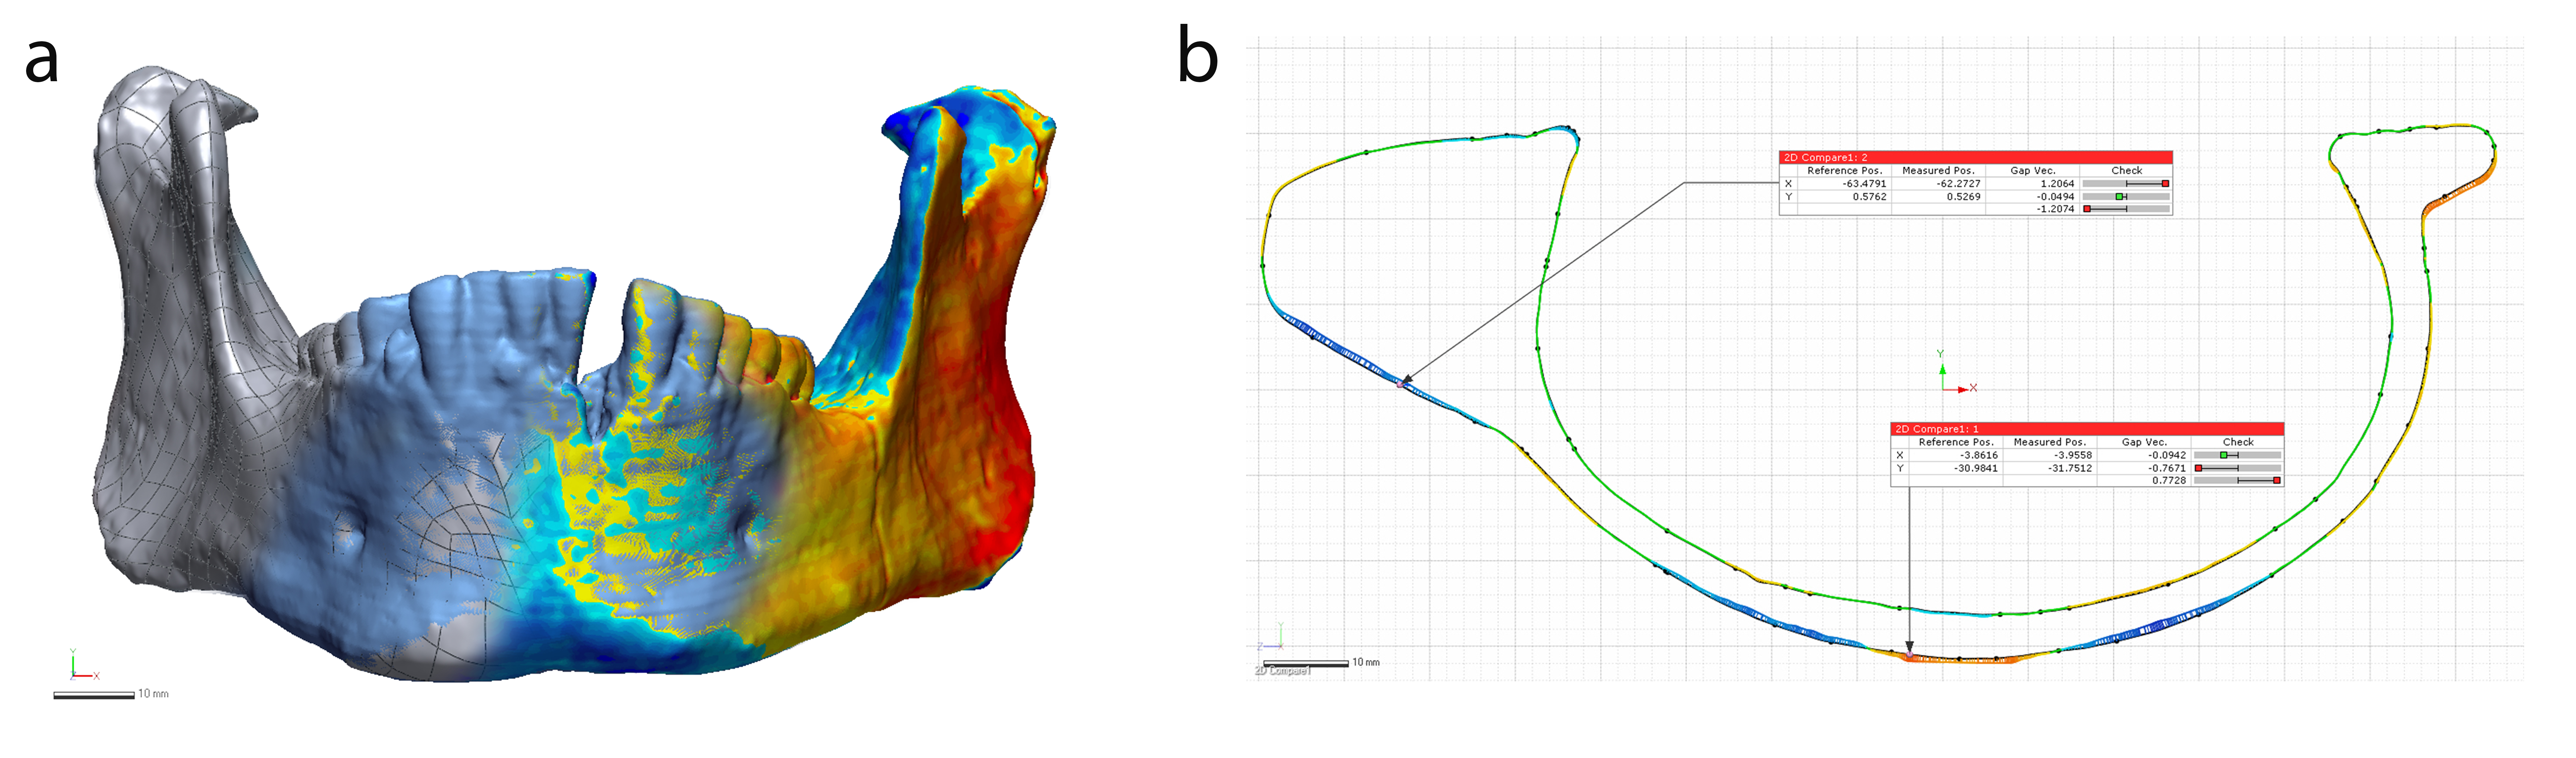
\includegraphics[width=\linewidth]{Fig2}
\caption{3D Compare (a) illustrates the nominal data (left), paired points from nominal data/point cloud (center), and gap distances (right) for UCB-6B36-B34-2-15925 (\textit{Note: inspection parameters were altered to more dramatically illustrate gap distances in this figure}), and 2D Compare (b) illustrates gap distances for a single cross-section for Caddo effigy vessel NSU-773.}
\label{fig:Fig2}
\end{figure}

The minimum and maximum call-outs include the highest deviations for the part overall or for a cluster selection of the part. This process differs from the gap distance in that gap distances are the deviations between the reference and measured data at a particular location. The histogram shown in each of the following figures illustrates the Gaussian distribution for the number of errors over the whole deviation. The graph is split into six segments: 1-Sigma at 31 percent from the average to the maximum deviation in each direction, 2-Sigma at 69 percent from the average to the maximum deviation in each direction, and 3-Sigma at 93.3 percent from the average to the maximum deviation in each direction. The AVG (average) is the sum of all deviations divided by the number of all deviations, and the RMS is the square root of all squared deviations divided by the number of all deviations (sometimes referred to as the effective deviation). In Tol and Out Tol percentages indicate the percentage of deviations in or out of a given tolerance, and Over Tol and Under Tol percentages indicate the percentage of deviations over (positive direction) or under (negative direction) the tolerance range by the mesh normal of the reference mesh.

\section*{Results}

Figure ~\ref{fig:Fig2} illustrates the nominal data, point cloud, and gap distances populated for an analysis of the mandible. Comparisons are limited to the topology of the nominal data due to the fact that some of the prints are representative of a single component of a larger object. It is, however, possible to compare each mesh by limiting the analysis to the topology of the nominal data, ensuring that internal structures and/or scaffolding were excluded from the inspection process \citep{RN5940}.

\subsection*{Modern human mandible (UCB-6B36-B34-2-15925)}

The 3D print of the modern human (\textit{Homo}) mandible was 43.3471 percent in tolerance ($\pm$ 0.1 mm), with 43.6886 percent of the print over tolerance, and 12.9643 percent under (Figure ~\ref{fig:FigMandible}). Areas surrounding the left and right rami---to include the temporal crests, mandibular notches, and condylar processes---appear to have warped slightly outward, as interior areas are under tolerance, and exterior areas are over (Supplemental Information). Further, the left molars and areas of the alveolar yokes appear slightly above tolerance.

\begin{figure}[ht]\centering
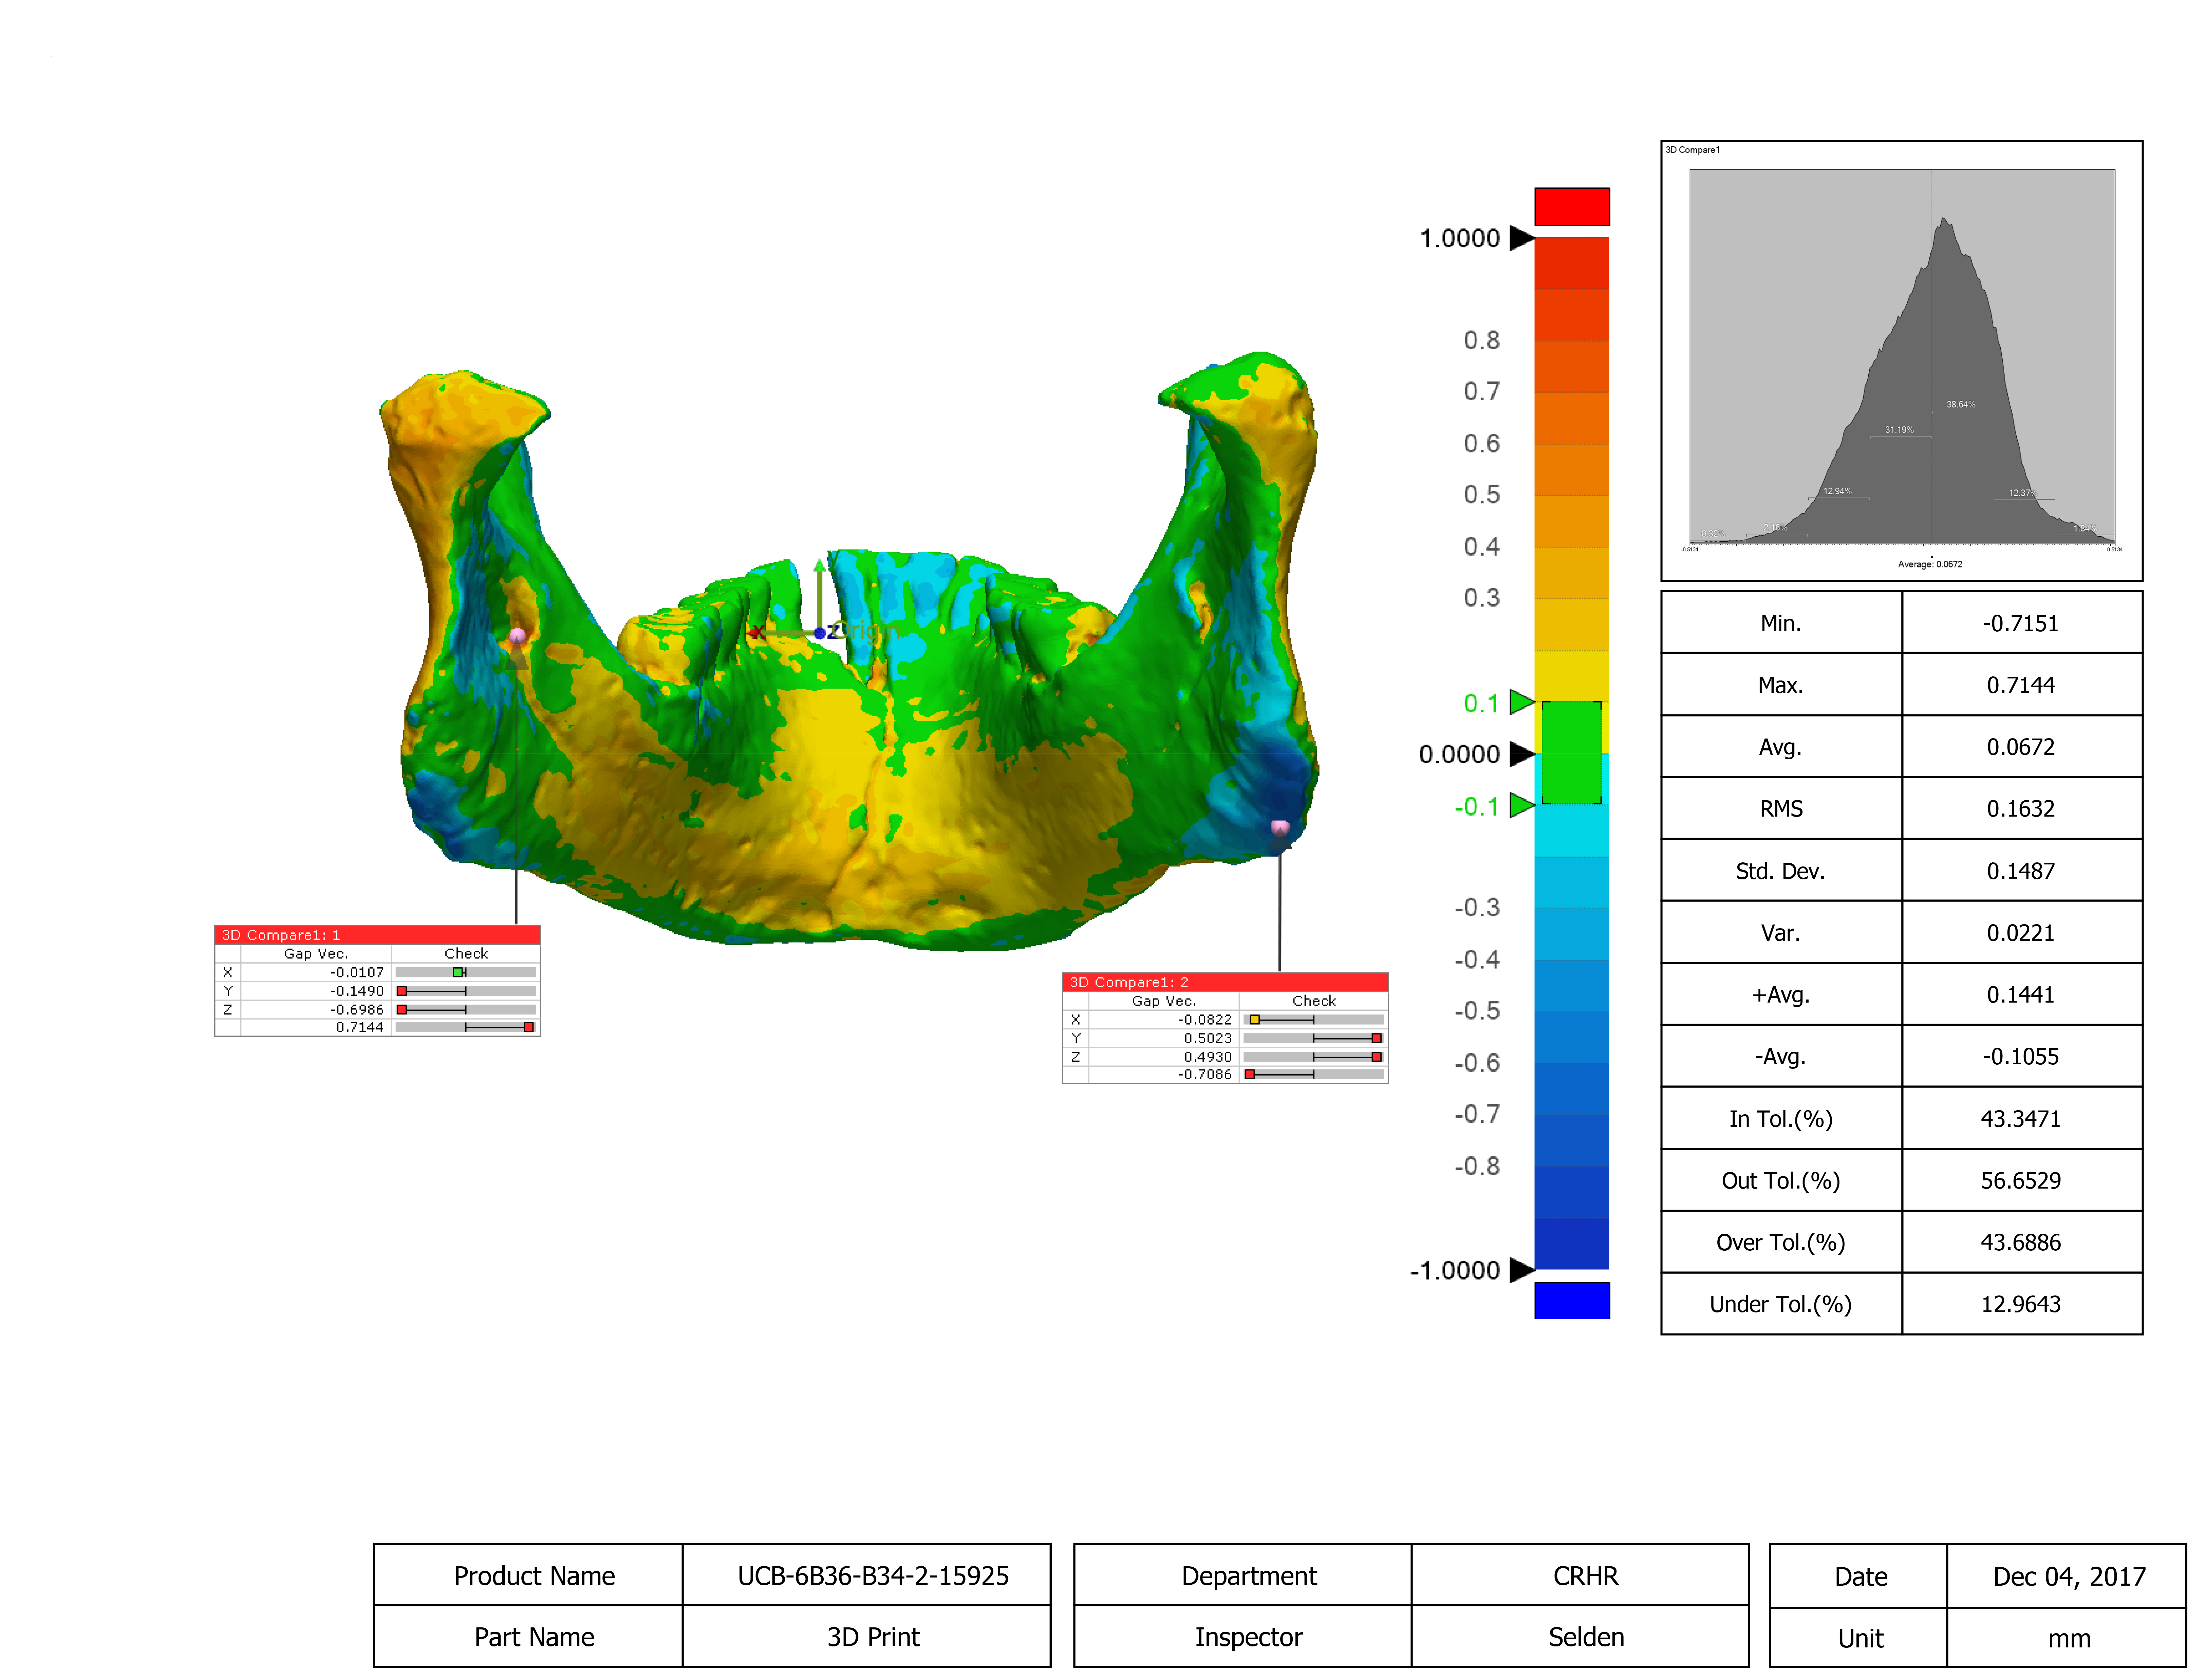
\includegraphics[width=\linewidth]{FigMandible}
\caption{3D compare results of nominal and measured data for UCB-6B36-B34-2-15925. Areas in green reflect the geometry of the mandible that is in tolerance. Call-outs were issued for the maximum above/below gap distances for each.}
\label{fig:FigMandible}
\end{figure}

The 2D compare results (Supplementary Information) similarly demonstrate the gap distances associated with a single section. For 2D Compare 1, which sectioned the mandible from the mental foramina to the angle, the rear of the 3D print demonstrates more variability. Overall, 42.7079 percent of the 2D Compare 1 section was in tolerance with 51.9764 percent over and 5.3158 percent under. The maximum distance in 2D Compare 1 was 0.5081 mm, and the minimum was -0.9622 mm.

In an effort to further clarify the gap distances associated with the rear of the mandible, 2D Compare 2 runs from the base of the mandibular body near the angle to the mandibular notch. The outer areas of this section were often above tolerance, where the internal areas were more regularly below. Overall, 28.4483 percent of the 2D Compare 2 section was in tolerance with 42.4808 percent over and 29.0709 percent under. The maximum distance in 2D Compare 2 was 0.5823 mm, and the minimum was -1.2724 mm.

The next section (2D Compare 3) runs from the base of the area near the mental protuberance to the top of the dental arcade (Supplementary Information). Overall, 43.1644 percent of the 2D Compare 3 section was in tolerance with 42.4731 percent over tolerance and 14.3625 percent under. The maximum distance in 2D Compare 3 was 0.4961 mm, and the minimum was -0.2289 mm.

The last section (2D Compare 4) encircles the dental arcade and the rami; however, it should be noted that the whole of the dental arcade is not captured at the alveolar yoke. Overall, 37.4746 percent of the 2D Compare 4 section was in tolerance with 47.4272 percent over and 15.0982 percent under. The maximum distance in 2D Compare 4 was 0.5053 mm, and the minimum was -0.7668 mm.

\subsection*{Clovis wrench (ASM A-32640)}

The 3D print of the Clovis wrench---a bone tool---was found to be 28.3637 percent in tolerance (Figure ~\ref{fig:FigWrench}), with 62.2274 percent of the print over tolerance, and 9.4089 percent under tolerance. Those areas of the print near the closed-end of the wrench include the highest deviations. The maximum distance in the 3D Compare was 1.1697 mm, and the minimum was -1.1495 mm.

\begin{figure}[ht]\centering
\includegraphics[width=\linewidth]{FigWrench}
\caption{3D compare results of nominal and measured data for ASM A-32640. Areas in green reflect the geometry of the artifact that is in tolerance. Call-outs were issued for the maximum above/below gap distances for each.}
\label{fig:FigWrench}
\end{figure}

In an effort to further clarify gap distances, 11 2D Compare sections were collected along the long (Y-) axis of the wrench (Supplementary Information). One final section, 2D Compare 12, runs from the closed-end of the wrench to the base. Overall, 26.3471 percent of the 2D Compare 12 section was in tolerance with 64.9486 percent over and 8.7043 percent under. The maximum distance in 2D Compare 12 was 1.1594 mm, and the minimum was -0.355 mm.

\subsection*{Caddo effigy bowl (rounded base) (NSU-773)}

The 3D print of Caddo effigy bowl NSU-773 was found to be 50.1606 percent in tolerance (Figure ~\ref{fig:FigTurtle}), with 30.5019 percent of the print over, and 19.3374 percent under tolerance. Those areas of the print near the base, and on the bottom of the tab tail of the vessel include the highest deviations. The maximum distance in the 3D Compare was 1.0223 mm, and the minimum was -1.024 mm. 

\begin{figure}[ht]\centering
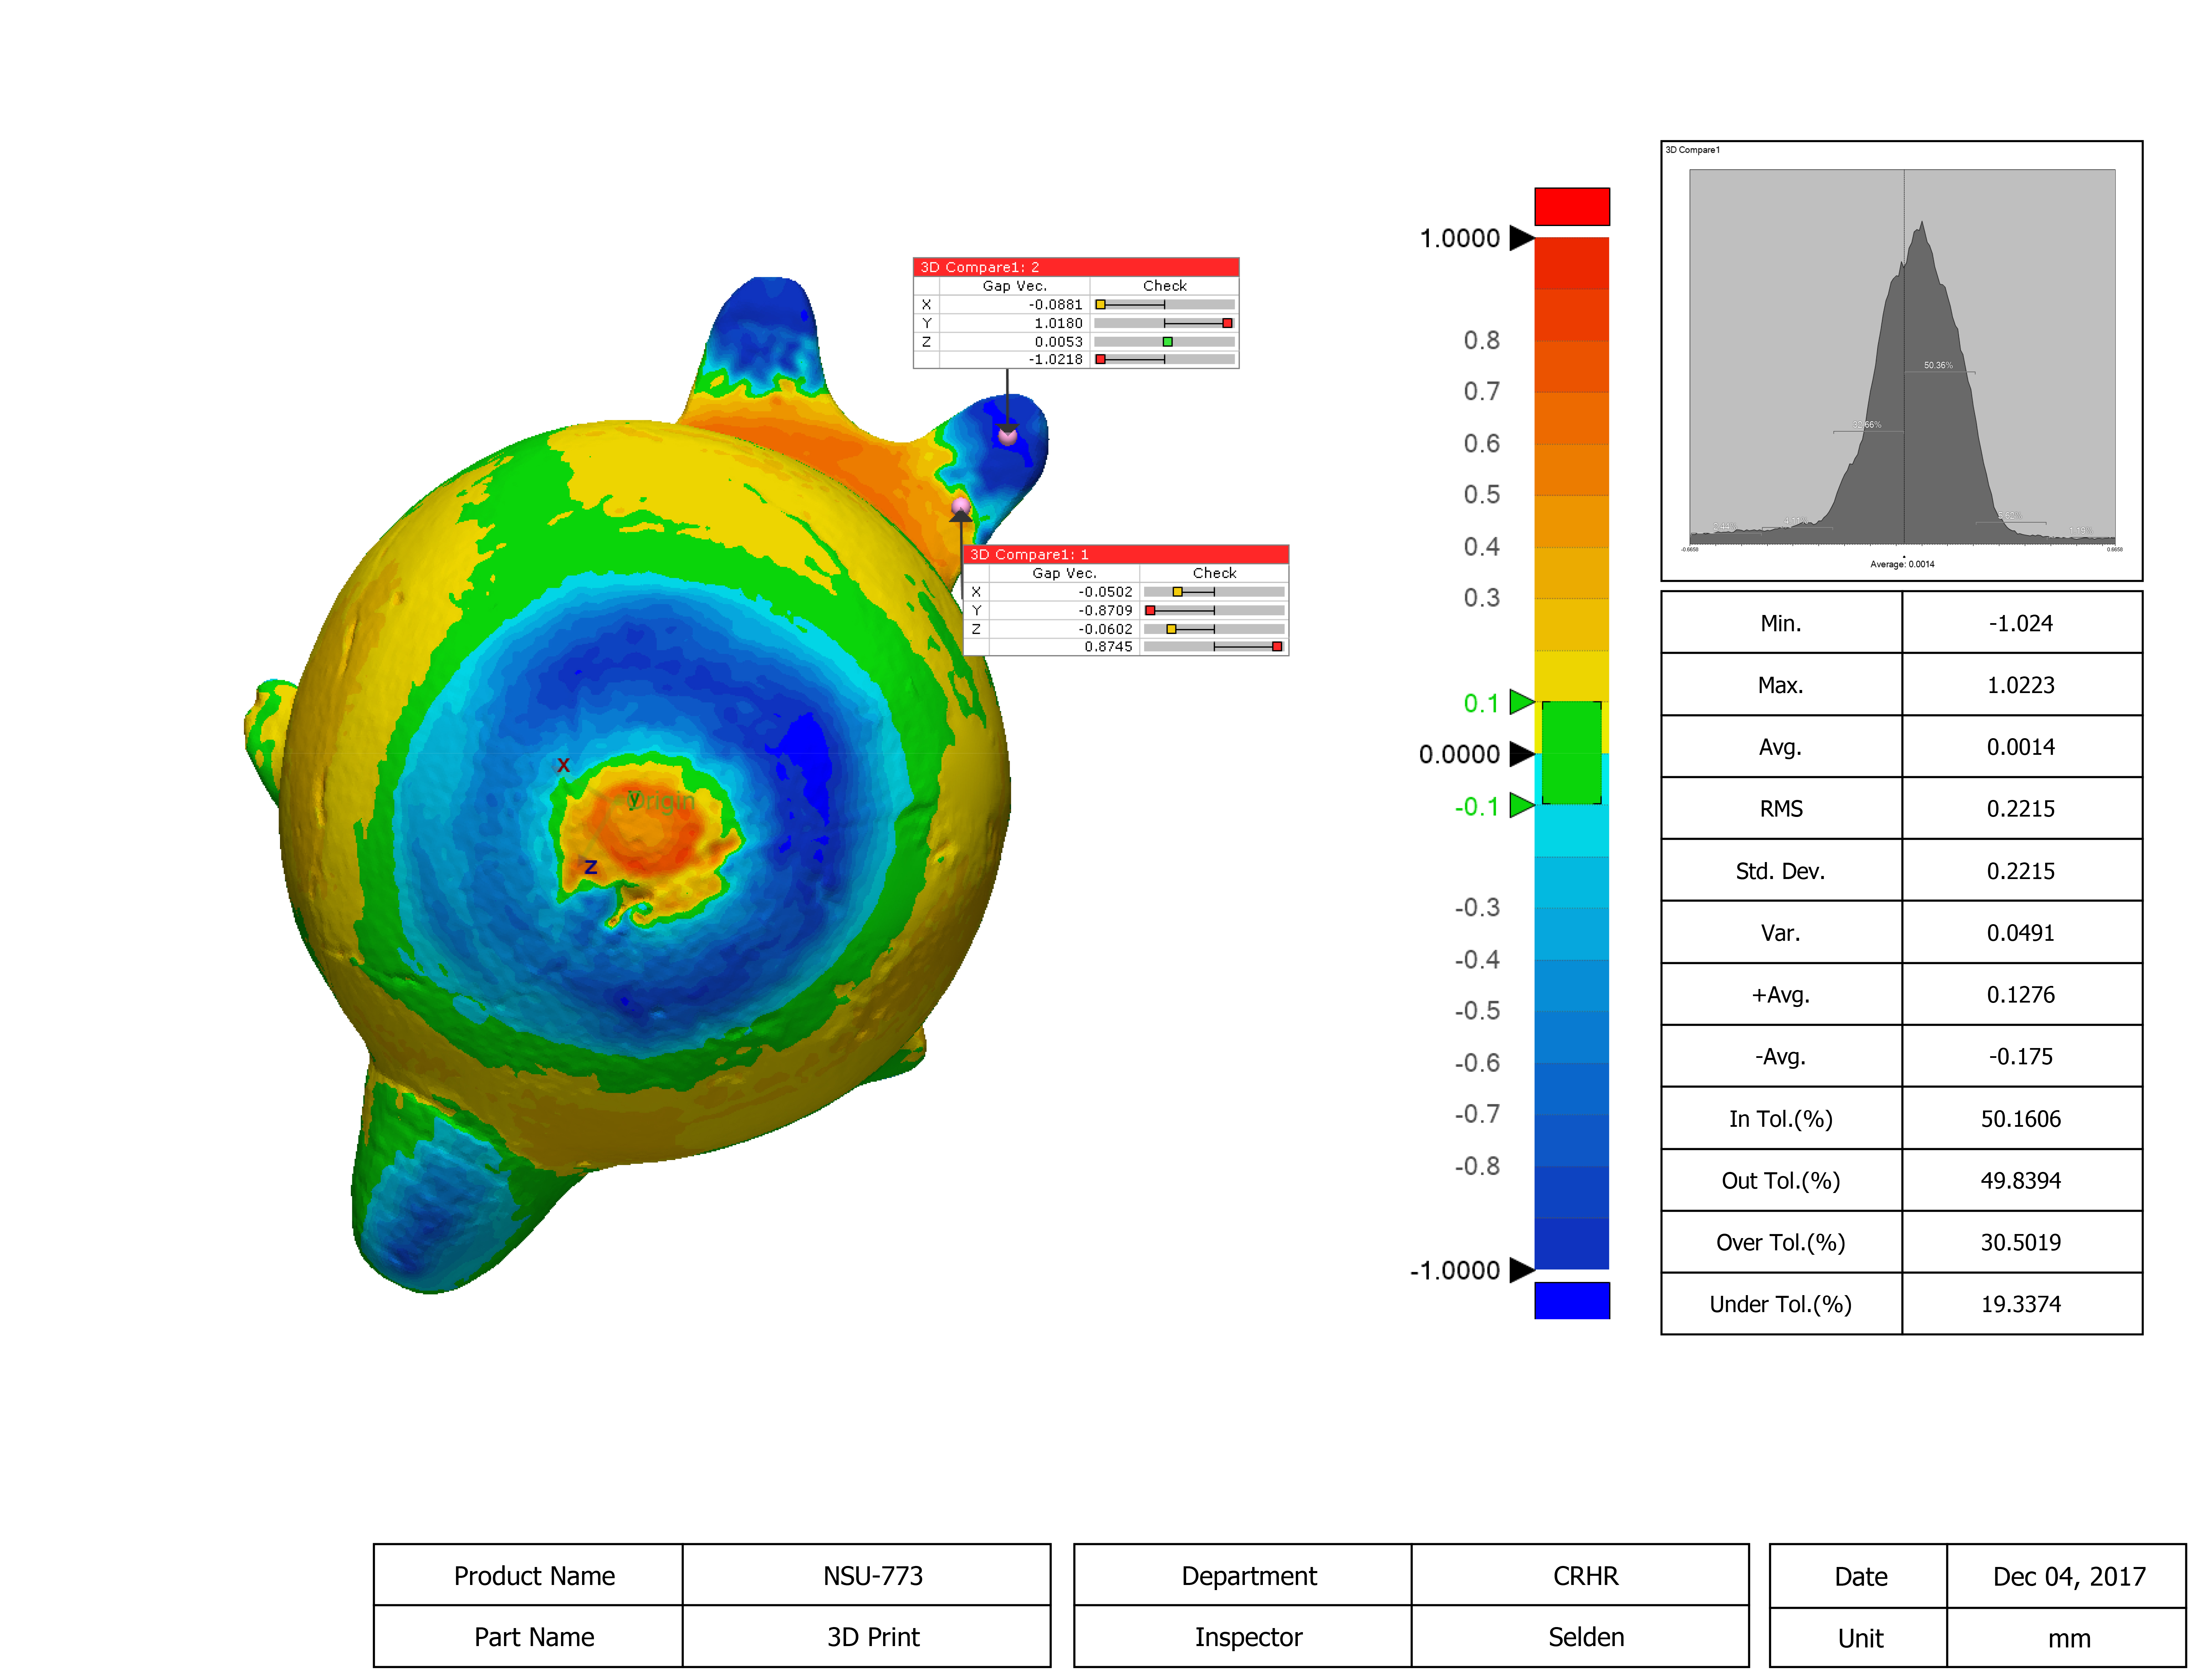
\includegraphics[width=\linewidth]{FigTurtle}
\caption{3D compare results of nominal and measured data for NSU-773. Areas in green reflect the geometry of the artifact that is in tolerance. Call-outs were issued for the maximum above/below gap distances for each.}
\label{fig:FigTurtle}
\end{figure}

The vessel was sectioned from the tip of the effigy head to the center of the tab tail (2D Compare 1). Overall, 40.4971 percent of 2D Compare 1 was in tolerance, with 34.6772 percent over and 24.8257 percent under tolerance. The maximum distance was 0.7843 mm, and the minimum was -1.003 mm.

An additional section (2D Compare 2) was collected along the axis associated with the effigy's appendages. Overall, 39.2786 percent of 2D Compare 2 was in tolerance, with 29.9247 percent over and 30.7967 percent under tolerance. The maximum distance was 0.3913 mm, and the minimum was -0.9747 mm.

\subsection*{Caddo effigy bowl (flat base) (41UR2-23)}

The 3D print of Caddo effigy bowl 41UR2-23 was found to be 53.9231 percent in tolerance (Figure ~\ref{fig:FigDeer}), with 40.4989 percent of the print over, and 5.578 percent under tolerance. The area of the print near the base includes the highest gap distances. The maximum distance in the 3D Compare was 0.7405 mm, and the minimum was -0.5369 mm.

\begin{figure}[ht]\centering
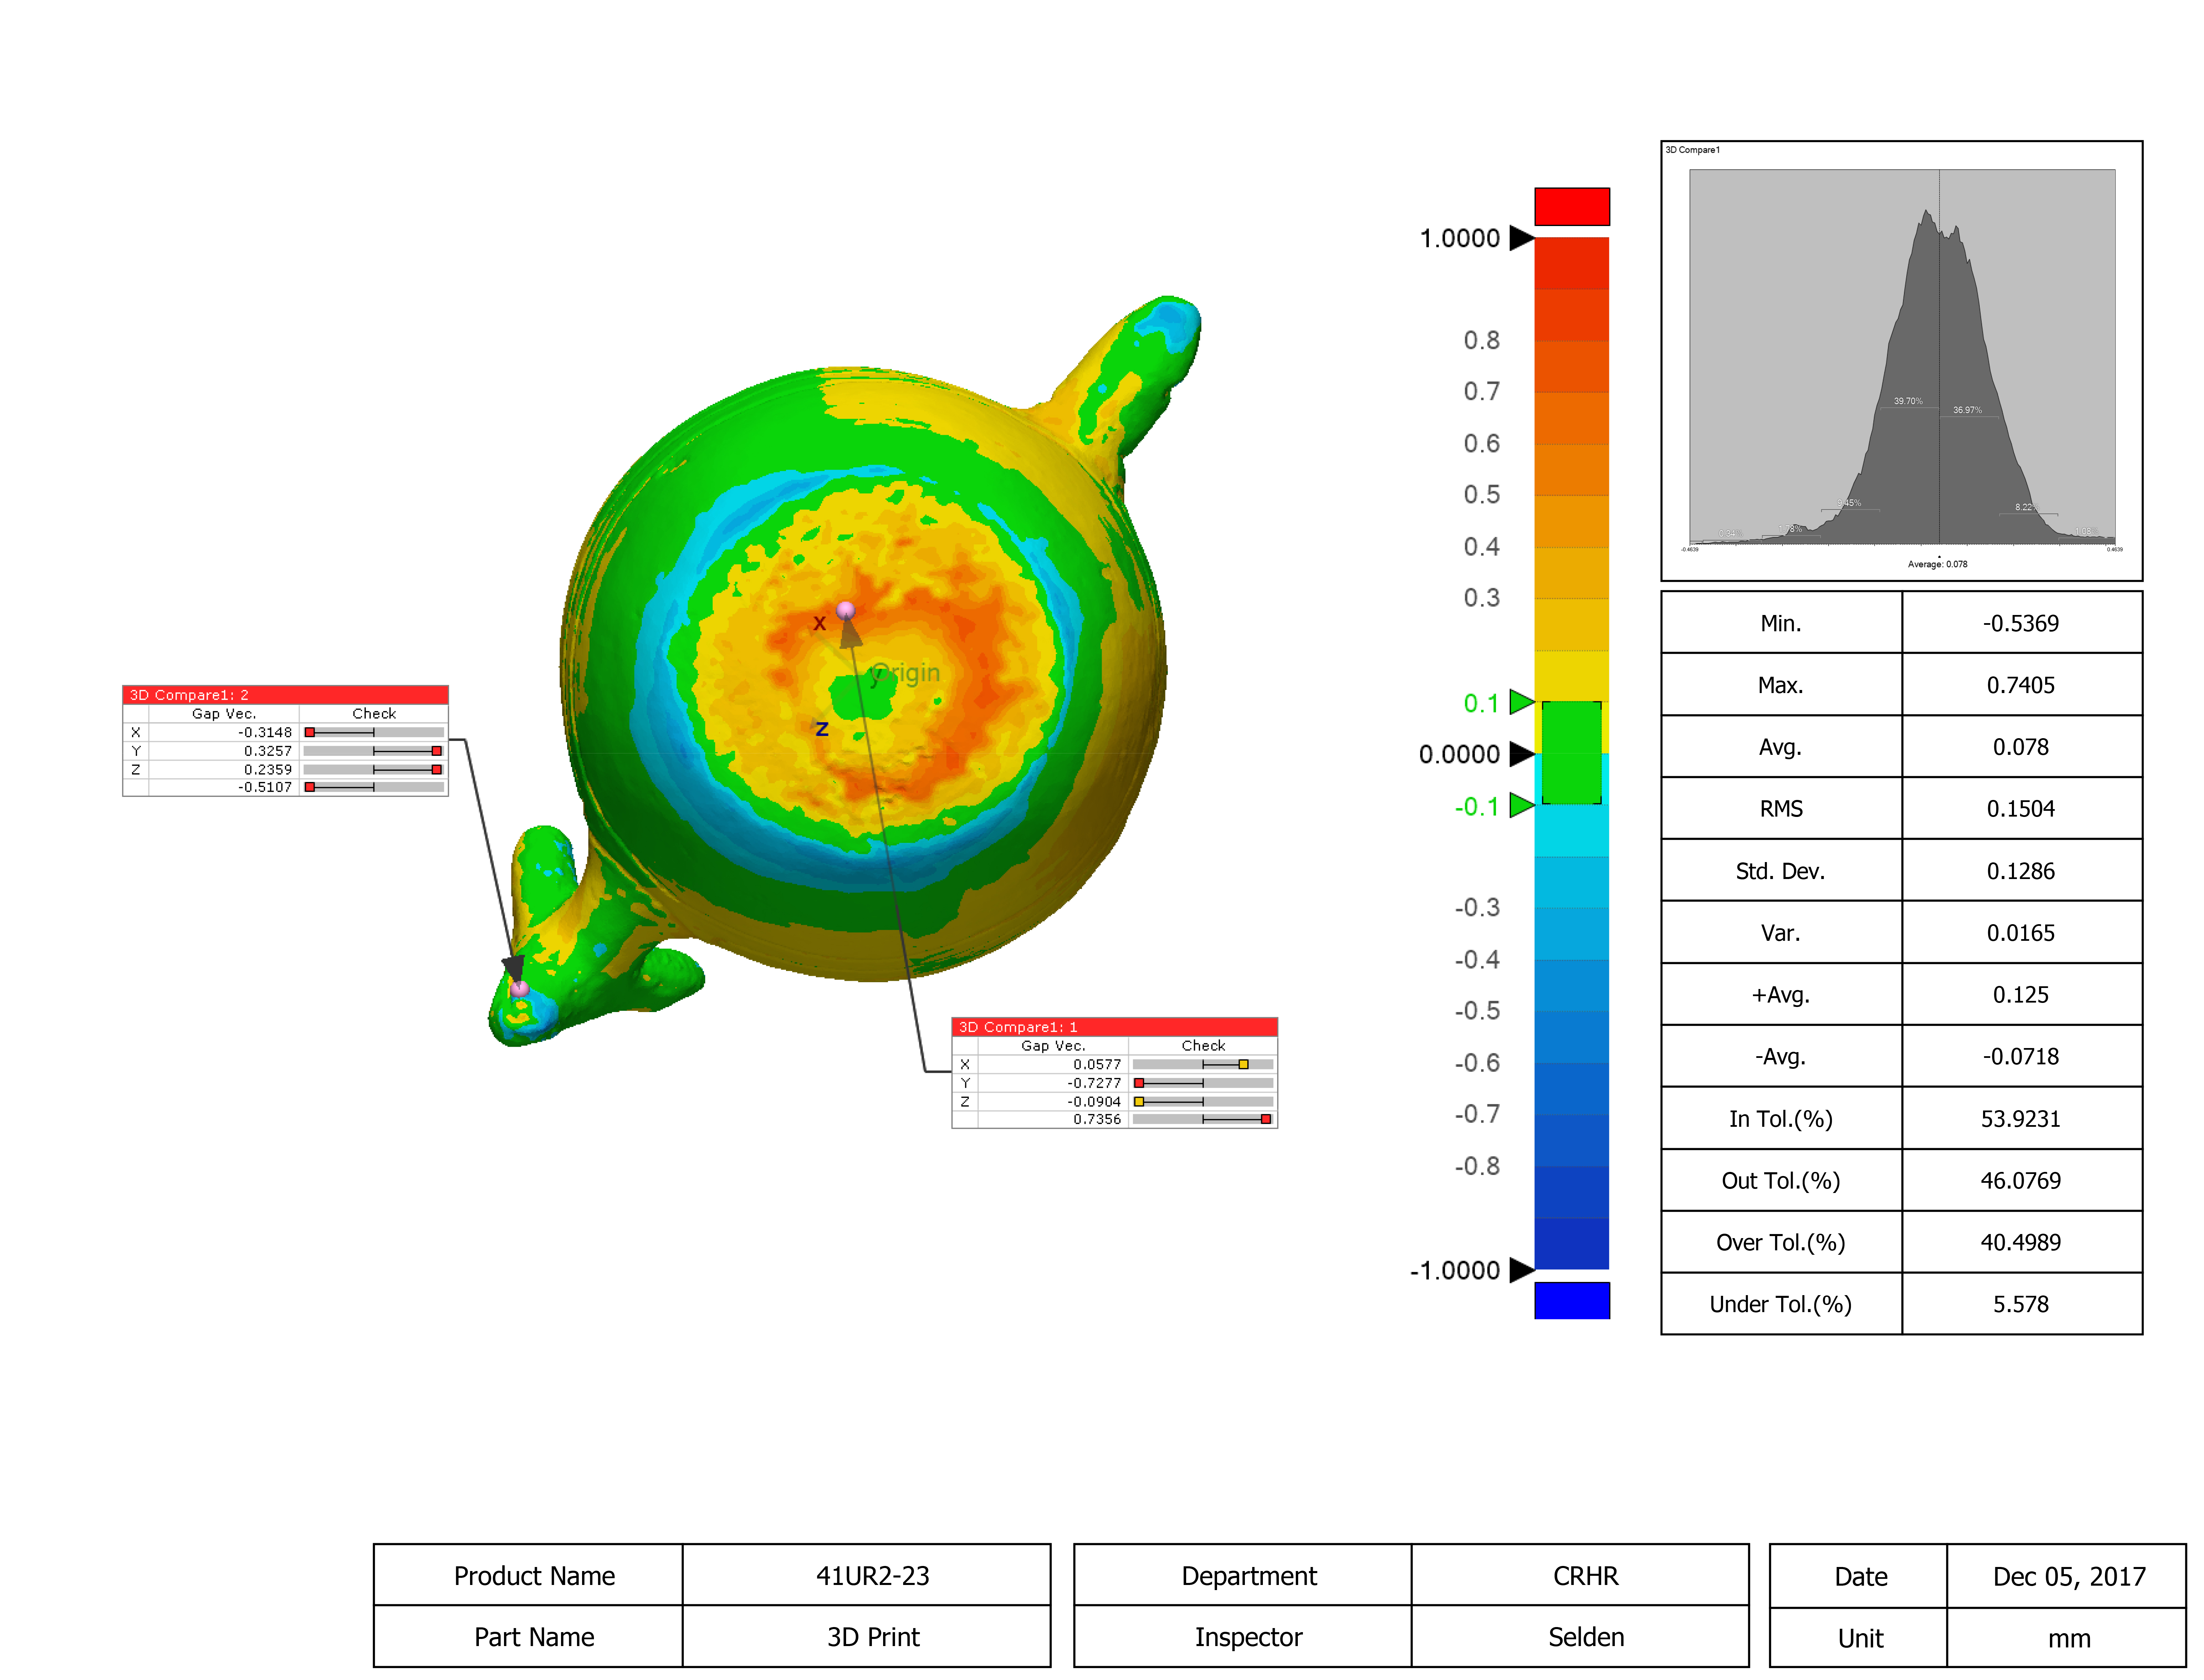
\includegraphics[width=\linewidth]{FigDeer}
\caption{3D compare results of nominal and measured data for 41UR2-23. Areas in green reflect the geometry of the artifact that is in tolerance. Call-outs were issued for the maximum above/below gap distances for each.}
\label{fig:FigDeer}
\end{figure}

The first section (2D Compare 1) was collected near the mid-line of the vessel. Overall, 49.5912 percent of 2D Compare 1 was in tolerance, with 44.1537 percent over, and 6.2551 percent under tolerance. The maximum distance was 0.8323 mm, and the minimum was -0.3088.

The second section (2D Compare 2) was collected from the tip of the effigy head to the tip of the tail. Overall, 53.6955 percent of 2D Compare 2 was in tolerance, with 39.2166 percent over, and 7.0879 percent under tolerance. The maximum distance was 0.658 mm, and the minimum was -0.3078 mm.

\subsection*{Clovis preform (TARL-41UV2-908-1258)}

The 3D print of the Clovis preform from the Kincaid site (TARL-41UV2-908-1258) was found to be 36.8608 percent in tolerance (Figure ~\ref{fig:FigPreform}), with 56.7688 percent of the print over, and 6.3704 percent under tolerance. Those areas of the print near the edges, and near the removal closest to the base include the highest gap distances. The maximum distance in the 3D Compare was 1.035 mm, and the minimum was -1.0253 mm.

\begin{figure}[ht]\centering
\includegraphics[width=\linewidth]{FigPreform}
\caption{3D compare results of nominal and measured data for TARL-41UV2-908-1258. Areas in green reflect the geometry of the artifact that is in tolerance. Call-outs were issued for the maximum above/below gap distances for each.}
\label{fig:FigPreform}
\end{figure}

In an effort to further clarify gap distances, 10 2D Compare sections were collected along the long (Y-) axis of the wrench (Supplementary Information). One final section, 2D Compare 11, runs from the point to the base. Overall, 32.1765 percent of the 2D Compare 11 section was in tolerance with 67.08235 percent over and 0.9771 percent under. The maximum distance in 2D Compare 11 was 1.1336 mm, and the minimum was -0.1476 mm.

\section*{Discussion}

Gap distances that occur between the original scan data and the 3D printed replicas were illustrated. In addition to the 3D Compare results, 2D compare results were employed to illustrate the variability in specific sections of the replicas. Results help to clarify the range and character of the deviations that occur between printed replicas and the meshes used to produce them. Additional implications for these results include the refinement of work flows associated with 3D printing, and the refinement of printed replicas using computer aided inspection to guide finishing decisions.

\subsection*{3D/2D Compare}

The 3D compare results demonstrate the variegated results produced by the printer, for which the in-tolerance results ranged from 28.3637 to 53.9231 percent (Table ~\ref{tab:Tbl1}). All meshes had a higher OverTol percentage. In future iterations of the inspection protocol, it may be worth including a measure of thickness to explore whether those areas found to be under tolerance on one side of the object are over tolerance on the opposing side, which may indicate some degree of warping during the printing process. 

\begin{table}[tbh]\centering
\footnotesize
\caption{Results of 3D comparison between the nominal and measured data.}
\centering
\begin{tabular}{lcccc}
\hline
Specimen & InTol (\%) & OutTol (\%) & OverTol (\%) & UnderTol (\%)\\
\hline
UCB-6B36-B34-2-15925 & 43.3471 & 56.6529 & 43.6886 & 12.9643\\
ASM A-32640 & 28.3637 & 71.6363 & 62.2274 & 9.4089\\
NSU-773 & 50.1606 & 49.8394 & 30.5019 & 19.3374\\
TARL-41UR2-23 & 53.9231  & 46.0769 & 40.4989 & 5.578\\
TARL-41UV2-908-1258 & 36.8608 & 63.1392 & 56.7688 & 6.3704\\
\hline
\end{tabular}
\label{tab:Tbl1}
\end{table}

The combined 2D/3D Compare results (Figure ~\ref{fig:Fig3DCompare}) help to better characterize the variation that occurs in each of these six replicas. The subjective process of finishing could also be guided by the results of computer-aided inspections. While scaffolding was removed from the replicas used in this study, additional modifications were not undertaken due to the highly subjective nature (art) of finishing. Computer aided inspection could aid in the finishing process by pointing out areas of the replica that are over tolerance, and warrant touch-up (whether by Dremel, flex-shaft, sanding, or other means). For all but one of the prints (UCB-6B36-B34-2-15925), those areas with the highest gap distances include regions of the prints where scaffolding was attached. However, touch-ups (finishing) should only be applied on areas of the replica that are over-tolerance. 

\begin{figure}[ht]\centering
\includegraphics[width=\linewidth]{Fig3DCompare}
\caption{Composite of the 3D/2D compare results for the nominal and measured data for TARL-41UV2-908-1258.}
\label{fig:Fig3DCompare}
\end{figure}

\subsection*{Ancillary observations}

Results indicate that some prints are more true to form than others. Two replicas---one of the mandible, and the other of the Clovis preform---failed during the initial print, resulting in the need for a second print (those used in this study). Another possible avenue of gainful inquiry may be to print multiples of each replica to explore deviations for a single replica to identify any issues with replicability. This latter approach may be particularly useful for those wishing to incorporate 3D printed replicas in classroom- or laboratory-based activities. Many practitioners also paint the printed replicas, and it may be the case that some paints and stains---particularly when applied in multiple coats---may further alter the replica's morphology.

With regard to the refinement of work flows, inspections could be used to iteratively identify printer settings that result in the most accurate prints possible for a specific printer. While not explored here, the use of computer aided inspection might be used to test variable settings associated with printing; for instance, by printing the same replica at variable resolutions to identify accuracy versus time investment. Given the differential environments where printers are employed, an iterative refinement process could be used to identify the optimal settings for a specific printer in a specific location (accounting for variabilities in local temperature, humidity, etc). 

\section*{Conclusion}

This analysis was aimed at the inspection of 3D prints for six specimens related to cultural heritage with the goal of identifying and characterizing the variability that occurs between the original mesh and printed replicas prior to their distribution to students and workshop participants to collect orthogonal measurements. Through the use of 3D and 2D Compare analyses in Geomagic Control X, the character of the gap distances between nominal and measured data was further clarified. Ancillary avenues of inquiry were identified and include (1) the systematic, iterative refinement of those settings that can be used to consistently generate the most accurate 3D print possible; and (2) the possible utility of computer aided inspection in the finishing of printed and painted replicas. These lines of inquiry lie beyond the scope of this study; however, this study lays the foundation necessary for those pursuits.

\section*{Acknowledgments}

We express our gratitude to the Ralph W. Steen Library at Stephen F. Austin State University for providing access to the 3D printer, and to Lauren Butaric and Tad Britt for their comments and constructive criticisms on an earlier draft of this paper.

Thanks also to the Caddo Nation of Oklahoma, Arizona State Museum, Louisiana State Exhibit Museum, Department of Anthropology at the University of Colorado Boulder, and Texas Archeological Research Laboratory for the requisite permissions and access needed to collect these scan data. Funding for the scan of NSU-773 was provided to RZS by grant P14AP00138 from the National Center for Preservation Technology and Training. 

\section*{References Cited}

\bibliography{cai}

\end{document}